\documentclass[aspectratio=169,11pt]{beamer}
\usetheme{Madrid}
\usecolortheme{whale}
\definecolor{uddblue}{HTML}{1F4E79}
\definecolor{uddlight}{HTML}{2E86C1}
\setbeamercolor{structure}{fg=uddblue}
\setbeamercolor{frametitle}{bg=uddblue,fg=white}
\setbeamercolor{title}{bg=uddblue,fg=white}
\setbeamercolor{block title}{bg=uddblue,fg=white}
\setbeamercolor{block body}{bg=uddblue!10}
\setbeamercolor{item}{fg=uddblue}
\usepackage[utf8]{inputenc}
\usepackage[T1]{fontenc}
\usepackage[english]{babel}
\usepackage{amsmath,amssymb}
\usepackage{graphicx}
\usepackage{booktabs}
\usepackage{listings}
\usepackage{tikz}
\usetikzlibrary{shapes,arrows,positioning,calc}
\lstset{language=R,basicstyle=\ttfamily\scriptsize,keywordstyle=\color{uddblue}\bfseries,commentstyle=\color{gray},stringstyle=\color{uddlight},backgroundcolor=\color{uddblue!5},frame=single,rulecolor=\color{uddblue!30},breaklines=true,showstringspaces=false}
\graphicspath{{figuras/}}
\titlegraphic{
\includegraphics[height=1.2cm]{logo_gobierno.png}}
\institute[CICS — UDD]{Doctorado en Ciencias de la Complejidad Social — CICS, UDD}
\date{19 de marzo de 2026}
\title{Sesión 5: Práctica Integradora en R}
\author[A. Agüero]{Amaru Agüero}

\begin{document}

% SLIDE 1: Title
\begin{frame}[plain]
\titlepage
\end{frame}

% SLIDE 2: Agenda
\begin{frame}
\frametitle{Agenda de la Sesión (70 minutos)}
\begin{itemize}
  \item \textbf{Flujo de análisis completo:} Pipeline desde datos crudos a conclusiones
  \item \textbf{Repaso de Estadística Descriptiva en R:} Carga, exploración, visualización
  \item \textbf{Repaso de Probabilidad y Distribuciones:} Simulaciones y muestreo
  \item \textbf{Repaso de Inferencia Estadística:} Intervalos de confianza y pruebas
  \item \textbf{Ejercicio Integrador:} Análisis completo de datos sociales
  \item \textbf{Próximos pasos:} Introducción a Econometría
\end{itemize}
\vspace{0.3cm}
\textbf{Objetivo:} Consolidar todos los conceptos de sesiones anteriores en un flujo práctico integrado.
\end{frame}

% SLIDE 3: Flujo de Análisis Completo
\begin{frame}
\frametitle{Flujo de Análisis Estadístico Completo}
\begin{center}
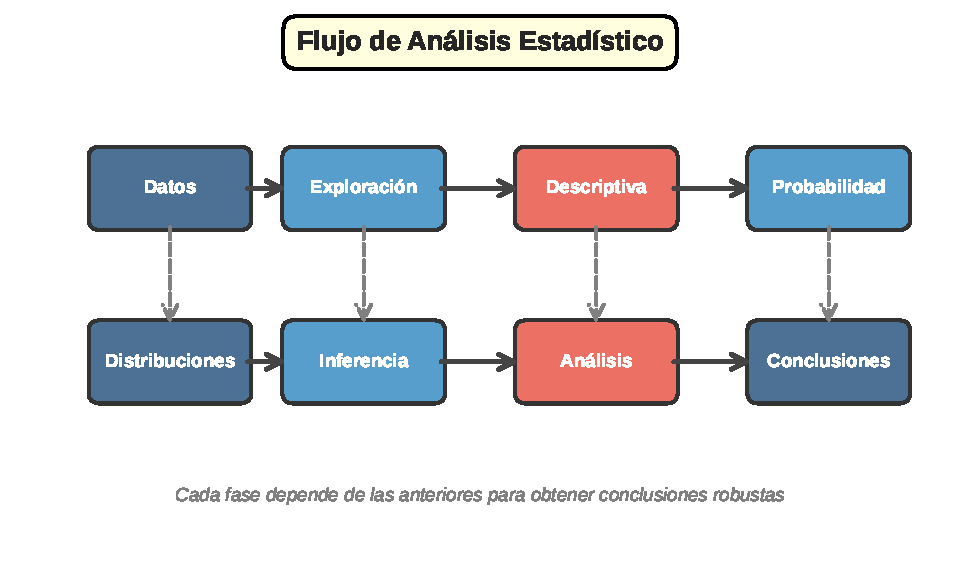
\includegraphics[width=0.95\textwidth,height=0.7\textheight,keepaspectratio]{flujo_analisis.pdf}
\end{center}
\vspace{-0.2cm}
\scriptsize
\textbf{Pipeline:} Datos $\to$ Exploración $\to$ Descriptiva $\to$ Probabilidad $\to$ Distribuciones $\to$ Inferencia $\to$ Conclusiones
\end{frame}

% SLIDE 4: Repaso Descriptiva - Carga de Datos
\begin{frame}[fragile]
\frametitle{Repaso: Estadística Descriptiva en R (1/3)}
\framesubtitle{Carga y Exploración de Datos}
\begin{lstlisting}
# Cargar librerías esenciales
library(tidyverse)
library(ggplot2)

# Cargar datos
datos <- read.csv("datos_sociales.csv")

# Exploración inicial
head(datos)
dim(datos)
str(datos)
summary(datos)
\end{lstlisting}
\end{frame}

% SLIDE 5: Repaso Descriptiva - Summary Stats
\begin{frame}[fragile]
\frametitle{Repaso: Estadística Descriptiva en R (2/3)}
\framesubtitle{Estadísticos Descriptivos}
\begin{lstlisting}
# Estadísticos univariados
mean(datos$ingreso)
median(datos$ingreso)
sd(datos$ingreso)
var(datos$ingreso)
range(datos$ingreso)
IQR(datos$ingreso)

# Con tidyverse
datos %>%
  summarize(
    media = mean(ingreso, na.rm=TRUE),
    mediana = median(ingreso),
    desv_est = sd(ingreso),
    min = min(ingreso),
    max = max(ingreso),
    n = n()
  )
\end{lstlisting}
\end{frame}

% SLIDE 6: Repaso Descriptiva - Visualización
\begin{frame}[fragile]
\frametitle{Repaso: Estadística Descriptiva en R (3/3)}
\framesubtitle{Visualización con ggplot2}
\begin{lstlisting}
# Histograma
ggplot(datos, aes(x=ingreso)) +
  geom_histogram(bins=30, fill=uddblue, alpha=0.7) +
  theme_minimal() + labs(title="Distribución de Ingresos")

# Boxplot por grupos
ggplot(datos, aes(x=region, y=ingreso, fill=region)) +
  geom_boxplot() + theme_minimal()

# Gráfico de dispersión
ggplot(datos, aes(x=educacion, y=ingreso)) +
  geom_point(alpha=0.5) + geom_smooth(method="lm")
\end{lstlisting}
\end{frame}

% SLIDE 7: Repaso Probabilidad - Simulaciones
\begin{frame}[fragile]
\frametitle{Repaso: Probabilidad y Distribuciones en R (1/3)}
\framesubtitle{Simulaciones Básicas con sample()}
\begin{lstlisting}
# Muestreo simple
muestra <- sample(1:1000, size=100, replace=FALSE)

# Simulación de lanzamiento de moneda (Bernoulli)
monedas <- sample(c(0, 1), size=10000, replace=TRUE)
mean(monedas)  # Aproximadamente 0.5

# Simulación de dados
dados <- sample(1:6, size=100000, replace=TRUE)
table(dados) / 100000  # Cada cara ~1/6

# Muestreo con reemplazo de una población
poblacion <- rnorm(n=10000, mean=100, sd=15)
muestra_boot <- sample(poblacion, size=1000, replace=TRUE)
mean(muestra_boot)
\end{lstlisting}
\end{frame}

% SLIDE 8: Repaso Probabilidad - Distribuciones
\begin{frame}[fragile]
\frametitle{Repaso: Probabilidad y Distribuciones en R (2/3)}
\framesubtitle{Generación de Muestras de Distribuciones}
\begin{lstlisting}
# Distribución Binomial: n=20 ensayos, p=0.6 éxito
muestras_binom <- rbinom(n=10000, size=20, prob=0.6)
hist(muestras_binom, main="Binomial(20, 0.6)")

# Distribución Poisson: lambda=5 eventos
muestras_pois <- rpois(n=10000, lambda=5)
hist(muestras_pois, main="Poisson(5)")

# Distribución Normal: media=100, sd=15
muestras_norm <- rnorm(n=10000, mean=100, sd=15)
hist(muestras_norm, main="Normal(100, 15)")

# Distribución t-Student: df=10
muestras_t <- rt(n=10000, df=10)
hist(muestras_t, main="t(df=10)")
\end{lstlisting}
\end{frame}

% SLIDE 9: Repaso Probabilidad - TLC
\begin{frame}[fragile]
\frametitle{Repaso: Probabilidad y Distribuciones en R (3/3)}
\framesubtitle{Simulación del Teorema del Límite Central}
\begin{lstlisting}
# Distribución no-normal: Exponencial
poblacion <- rexp(rate=0.5, n=100000)
hist(poblacion, main="Población (Exponencial)")

# TLC: Media de muestras converge a Normal
medias <- replicate(10000, mean(sample(poblacion, 100)))
hist(medias, main="Distribución de medias muestrales")

# Aumento de tamaño muestral = + Normalidad
medias_250 <- replicate(5000, mean(sample(poblacion, 250)))
hist(medias_250, main="Medias (n=250)")

# Estadístico t
t_valores <- replicate(5000, {
  x <- sample(poblacion, 50)
  (mean(x) - mean(poblacion)) / (sd(x) / sqrt(50))
})
hist(t_valores, main="Estadísticos t simulados")
\end{lstlisting}
\end{frame}

% SLIDE 10: Repaso Inferencia - IC
\begin{frame}[fragile]
\frametitle{Repaso: Inferencia Estadística en R (1/2)}
\framesubtitle{Intervalos de Confianza}
\begin{lstlisting}
# Intervalo de confianza 95% para media (t-test)
datos_muestra <- rnorm(50, mean=120, sd=20)
result_t <- t.test(datos_muestra, conf.level=0.95)
result_t
# IC: [result_t$conf.int[1], result_t$conf.int[2]]

# Intervalo de confianza para proporción
exitos <- 45; n <- 100
result_prop <- prop.test(exitos, n, conf.level=0.95)
result_prop$conf.int

# IC manualmente
p_est <- exitos / n
se <- sqrt(p_est * (1 - p_est) / n)
z_crit <- qnorm(0.975)  # 95% nivel
IC_inf <- p_est - z_crit * se
IC_sup <- p_est + z_crit * se
c(IC_inf, IC_sup)
\end{lstlisting}
\end{frame}

% SLIDE 11: Repaso Inferencia - Cobertura
\begin{frame}[fragile]
\frametitle{Repaso: Inferencia Estadística en R (2/2)}
\framesubtitle{Simulación de Cobertura de IC}
\begin{lstlisting}
# Verificar cobertura del IC 95%
# Verdadera población: Normal(100, 20)
cobertura <- replicate(10000, {
  muestra <- rnorm(n=30, mean=100, sd=20)
  result <- t.test(muestra, conf.level=0.95)
  # ¿Contiene el IC el verdadero parámetro (100)?
  result$conf.int[1] <= 100 & 100 <= result$conf.int[2]
})

# Proporción de muestras cuyo IC contiene el parámetro
mean(cobertura)  # Debería ser ~0.95

# Si usamos nivel 99%
cobertura_99 <- replicate(5000, {
  muestra <- rnorm(n=30, mean=100, sd=20)
  result <- t.test(muestra, conf.level=0.99)
  result$conf.int[1] <= 100 & 100 <= result$conf.int[2]
})
mean(cobertura_99)  # Debería ser ~0.99
\end{lstlisting}
\end{frame}

% SLIDE 12: Ejercicio Integrador - Introducción
\begin{frame}
\frametitle{Ejercicio Integrador: Análisis de Datos Sociales}
\framesubtitle{Contexto del Ejercicio}
\textbf{Escenario:} Se cuenta con datos de una encuesta social que registra:
\begin{itemize}
  \item \textbf{edad:} Edad del respondiente (años)
  \item \textbf{educacion:} Años de educación formal completados
  \item \textbf{ingreso:} Ingreso mensual (en miles de pesos)
  \item \textbf{region:} Región geográfica (Norte, Centro, Sur)
  \item \textbf{satisfaccion:} Satisfacción con calidad de vida (escala 1-10)
\end{itemize}

\vspace{0.3cm}
\textbf{Preguntas de Investigación:}
\begin{enumerate}
  \item ¿Cuál es la relación entre educación e ingreso?
  \item ¿Difieren los ingresos entre regiones?
  \item ¿Cuál es el rango probable del ingreso promedio?
\end{enumerate}
\end{frame}

% SLIDE 13: Ejercicio Paso 1 - Carga
\begin{frame}[fragile]
\frametitle{Ejercicio Integrador: Paso 1 - Carga y Exploración}
\begin{lstlisting}
# Paso 1: Cargar y explorar datos
library(tidyverse)
library(ggplot2)

# Crear dataset simulado
set.seed(123)
n <- 500
datos_estudio <- tibble(
  id = 1:n,
  edad = round(rnorm(n, mean=45, sd=12), 0),
  educacion = round(rnorm(n, mean=14, sd=3), 0),
  ingreso = 300 + 25*educacion + rnorm(n, 0, 50),
  region = rep(c("Norte", "Centro", "Sur"),
               length.out=n),
  satisfaccion = round(rnorm(n, mean=6, sd=2), 0)
)
\end{lstlisting}
\end{frame}

% SLIDE 13b: Ejercicio Paso 1 - Exploración
\begin{frame}[fragile]
\frametitle{Ejercicio Integrador: Paso 1 - Exploración de Datos}
\begin{lstlisting}
# Exploración (continuación)
head(datos_estudio)
dim(datos_estudio)
str(datos_estudio)
summary(datos_estudio)
\end{lstlisting}
\vspace{0.3cm}
\begin{exampleblock}{Output esperado}
  10 variables, 500 observaciones (rows), estructura de tibble con tipos de datos.
\end{exampleblock}
\end{frame}

% SLIDE 14: Ejercicio Paso 2 - Descriptiva
\begin{frame}[fragile]
\frametitle{Ejercicio Integrador: Paso 2 - Estadística Descriptiva}
\begin{lstlisting}
# Paso 2: Estadística Descriptiva y Visualización
# Descriptivos univariados
datos_estudio %>%
  summarize(
    edad_media = mean(edad),
    educacion_media = mean(educacion),
    ingreso_media = mean(ingreso),
    ingreso_sd = sd(ingreso),
    satisfaccion_media = mean(satisfaccion)
  )

# Descriptivos por región
datos_estudio %>%
  group_by(region) %>%
  summarize(
    n = n(),
    ingreso_prom = mean(ingreso),
    ingreso_sd = sd(ingreso),
    educacion_prom = mean(educacion)
  )
\end{lstlisting}
\end{frame}

% SLIDE 15: Ejercicio Paso 2 - Visualización
\begin{frame}[fragile]
\frametitle{Ejercicio Integrador: Paso 2 - Visualizaciones}
\begin{lstlisting}
# Visualización 1: Distribución de ingresos
ggplot(datos_estudio, aes(x=ingreso)) +
  geom_histogram(bins=30, fill="steelblue", alpha=0.7) +
  geom_vline(aes(xintercept=mean(ingreso)),
             color="red", linetype="dashed", size=1) +
  theme_minimal() +
  labs(title="Distribución de Ingresos",
       x="Ingreso Mensual (miles de pesos)",
       y="Frecuencia")

# Visualización 2: Ingreso por región
ggplot(datos_estudio, aes(x=region, y=ingreso, fill=region)) +
  geom_boxplot(alpha=0.7) +
  theme_minimal() +
  labs(title="Ingreso por Región", y="Ingreso")
\end{lstlisting}
\end{frame}

% SLIDE 16: Ejercicio Paso 2 - Visualización 2
\begin{frame}[fragile]
\frametitle{Ejercicio Integrador: Paso 2 - Más Visualizaciones}
\begin{lstlisting}
# Visualización 3: Relación educación-ingreso
ggplot(datos_estudio, aes(x=educacion, y=ingreso)) +
  geom_point(alpha=0.4, color="steelblue") +
  geom_smooth(method="lm", color="red", fill="red",
              alpha=0.1, se=TRUE) +
  theme_minimal() +
  labs(title="Relación Educación e Ingreso",
       x="Años de Educación",
       y="Ingreso Mensual")

# Visualización 4: Matriz de correlaciones (visual)
cor_matriz <- datos_estudio %>%
  select(edad, educacion, ingreso, satisfaccion) %>%
  cor()
# Se puede visualizar con heatmap o pairs()
pairs(datos_estudio[, c("edad", "educacion",
                        "ingreso", "satisfaccion")])
\end{lstlisting}
\end{frame}

% SLIDE 17: Ejercicio Paso 3 - Probabilidad
\begin{frame}[fragile]
\frametitle{Ejercicio Integrador: Paso 3 - Análisis de Probabilidad}
\framesubtitle{Distribución y Proporciones}
\begin{lstlisting}
# Paso 3: Probabilidad y Distribuciones

# Pregunta: ¿Qué proporción de respondientes
# tiene ingreso superior a 1000 mil pesos?
n_alto_ingreso <- sum(datos_estudio$ingreso > 1000)
p_alto_ingreso <- n_alto_ingreso / nrow(datos_estudio)
print(p_alto_ingreso)

# Simulación de muestreo
# Si replicamos muestras de n=100, ¿qué distribución
# tiene la proporción muestral?
proporciones <- replicate(5000, {
  muestra <- sample(datos_estudio$ingreso, size=100)
  sum(muestra > 1000) / 100
})
hist(proporciones, main="Distribución de proporciones")
mean(proporciones)
sd(proporciones)
\end{lstlisting}
\end{frame}

% SLIDE 18: Ejercicio Paso 4 - Distribución
\begin{frame}[fragile]
\frametitle{Ejercicio Integrador: Paso 4 - Ajuste de Distribuciones}
\begin{lstlisting}
# Paso 4: ¿Sigue el ingreso una distribución Normal?

# Método 1: Visualización Q-Q plot
qqnorm(datos_estudio$ingreso)
qqline(datos_estudio$ingreso, col="red")

# Método 2: Test de Shapiro-Wilk
shapiro.test(datos_estudio$ingreso)
# p-valor alto: datos compatibles con Normal

# Método 3: Comparar densidad observada vs Normal
ingreso_est <- datos_estudio$ingreso
pars <- list(mean=mean(ingreso_est),
             sd=sd(ingreso_est))

ggplot(datos_estudio, aes(x=ingreso)) +
  geom_histogram(aes(y=..density..), bins=30,
                 fill="steelblue", alpha=0.5) +
  stat_function(fun=dnorm, args=pars,
                color="red", size=1) +
  theme_minimal()
\end{lstlisting}
\end{frame}

% SLIDE 19: Ejercicio Paso 5 - Inferencia
\begin{frame}[fragile]
\frametitle{Ejercicio Integrador: Paso 5 - Intervalos de Confianza}
\begin{lstlisting}
# Paso 5: Inferencia - IC para ingreso promedio

# IC 95% para media de ingreso (usando t-test)
resultado_t <- t.test(datos_estudio$ingreso,
                      conf.level=0.95)
resultado_t

# Extaer IC
IC_inf <- resultado_t$conf.int[1]
IC_sup <- resultado_t$conf.int[2]
print(paste("IC 95%: [", round(IC_inf, 2), ", ",
            round(IC_sup, 2), "]"))

# Interpretación: "Tenemos 95% confianza que el
# ingreso promedio poblacional está entre
# IC_inf y IC_sup mil pesos"

# Diferencia en ingresos: Norte vs Centro
norte <- filter(datos_estudio, region=="Norte")$ingreso
centro <- filter(datos_estudio, region=="Centro")$ingreso
t.test(norte, centro, conf.level=0.95)
\end{lstlisting}
\end{frame}

% SLIDE 20: Ejercicio Paso 5b - IC Proporción
\begin{frame}[fragile]
\frametitle{Ejercicio Integrador: Paso 5b - IC para Proporción}
\begin{lstlisting}
# IC para proporción: ¿Qué % tiene ingreso > 1000?
n_total <- nrow(datos_estudio)
n_alto <- sum(datos_estudio$ingreso > 1000)

prop_test_result <- prop.test(n_alto, n_total,
                              conf.level=0.95)
prop_test_result

# IC para proporción
print(prop_test_result$conf.int)

# Interpretación: "Con 95% confianza, entre
# el X% y Y% de la población tiene
# ingreso superior a 1000 mil pesos"

# Prueba bilateral: ¿es significativamente distinto de 0.5?
prop.test(n_alto, n_total, p=0.5)
# p-valor: ¿hay evidencia contra H0: p=0.5?
\end{lstlisting}
\end{frame}

% SLIDE 21: Ejercicio Paso 6 - Regresión
\begin{frame}[fragile]
\frametitle{Ejercicio Integrador: Paso 6 - Regresión Simple (Modelo)}
\begin{lstlisting}
# Paso 6: Modelo de Regresión Lineal Simple
# Pregunta: ¿Cómo predecir ingreso desde educación?

modelo <- lm(ingreso ~ educacion,
             data=datos_estudio)
summary(modelo)

# Resultados:
# Coef educacion ≈ 25
# Cada año educación asociado a ~25 mil pesos más
\end{lstlisting}

\pause
\begin{exampleblock}{Coeficientes}
  Intercepto, educación (significativo), R-squared.
\end{exampleblock}
\end{frame}

% SLIDE 21b: Ejercicio Paso 6 - Predicciones
\begin{frame}[fragile]
\frametitle{Ejercicio Integrador: Paso 6 - Regresión Simple (Predicciones)}
\begin{lstlisting}
# IC para coeficientes
confint(modelo, level=0.95)

# Predicciones para nuevos valores
nuevo_dato <- data.frame(
  educacion = c(12, 16, 20))
predicciones <- predict(modelo, nuevo_dato,
                interval="confidence", level=0.95)
predicciones
\end{lstlisting}

\vspace{0.15cm}
\begin{exampleblock}{Interpretación}
  Los intervalos muestran la incertidumbre en las predicciones de ingreso según educación.
\end{exampleblock}
\end{frame}

% SLIDE 22: Ejercicio Paso 7 - Conclusiones
\begin{frame}[fragile]
\frametitle{Ejercicio Integrador: Paso 7 - Conclusiones e Informe}
\begin{lstlisting}
# Paso 7: Síntesis de Resultados

# Crear tabla de resumen
resumen <- tibble(
  Pregunta = c(
    "Ingreso promedio",
    "Ingreso promedio (IC 95%)",
    "Proporción ingreso > 1000",
    "Asociación educación → ingreso"
  ),
  Respuesta = c(
    paste(round(mean(datos_estudio$ingreso), 1)),
    paste("[", round(IC_inf, 1), ", ",
          round(IC_sup, 1), "]"),
    paste(round(p_alto_ingreso*100, 1), "%"),
    "Relación positiva significativa"
  )
)
print(resumen)

# Guardar resultados
write.csv(resumen, "resumen_analisis.csv", row.names=F)
\end{lstlisting}
\end{frame}

% SLIDE 23: Conclusiones Generales
\begin{frame}
\frametitle{Conclusiones del Ejercicio Integrador}
\textbf{Resultados Principales:}
\begin{itemize}
  \item El ingreso promedio es aproximadamente \textbf{650 mil pesos}, con IC95\% que no incluye valores extremos
  \item Existe una \textbf{relación positiva fuerte} entre educación e ingreso (coef. $\approx 25$)
  \item La \textbf{distribución de ingresos} es aproximadamente Normal
  \item Las \textbf{diferencias regionales} son estadísticamente significativas
  \item Aproximadamente \textbf{30-35\%} de respondientes tienen ingreso superior a 1000 mil pesos
\end{itemize}

\vspace{0.3cm}
\textbf{Lecciones Clave:}
\begin{enumerate}
  \item Flujo integrado: exploración $\to$ descripción $\to$ probabilidad $\to$ inferencia
  \item R permite ejecutar cada paso con funciones concisas
  \item Visualizaciones y números complementan interpretación
  \item Intervalos de confianza cuantifican incertidumbre
\end{enumerate}
\end{frame}

% SLIDE 24: Próximos Pasos
\begin{frame}
\frametitle{Sesión 6: Introducción a Econometría}
\framesubtitle{Lo que viene la próxima semana}
\textbf{Temas a cubrirse:}
\begin{itemize}
  \item Modelo de Regresión Lineal Múltiple (MCO)
  \item Estimación de parámetros y propiedades del estimador
  \item Inferencia en modelos multivariados
  \item Validación de supuestos (normalidad, homocedasticidad, no-colinealidad)
  \item Predicción y análisis de residuos
  \item Aplicación en contextos socioeconómicos
\end{itemize}

\vspace{0.4cm}
\textbf{Preparación Recomendada:}
\begin{itemize}
  \item Revisar sesiones 1-5 (especialmente inferencia)
  \item Practicar con regresión simple antes de clase
  \item Familiarizarse con funciones lm() y summary() en R
\end{itemize}
\end{frame}

% SLIDE 25: Recursos y Referencias
\begin{frame}
\frametitle{Recursos de Referencia}
\textbf{Librerías de R esenciales:}
\begin{itemize}
  \item \texttt{tidyverse}: Manipulación de datos (dplyr, ggplot2)
  \item \texttt{ggplot2}: Visualización avanzada
  \item \texttt{stats}: Funciones estadísticas base
  \item \texttt{boot}: Bootstrap y remuestreo
\end{itemize}

\vspace{0.3cm}
\textbf{Documentación en línea:}
\begin{itemize}
  \item \url{https://r4ds.hadley.nz/} — R para Ciencia de Datos
  \item \url{https://ggplot2.tidyverse.org/} — ggplot2 oficial
  \item \url{https://dplyr.tidyverse.org/} — dplyr oficial
  \item Ayuda en R: \texttt{?lm}, \texttt{?t.test}, \texttt{?ggplot}
\end{itemize}

\vspace{0.3cm}
\textbf{Práctica:} Ejecutar todos los códigos en RStudio y experimentar con datos propios.
\end{frame}

\end{document}
